\subsubsection*{Design}
As seen in \cref{img:coredes} the core will consist of a block of memory, an ALU combined with the blitter, and several smaller single function cores.

The graphic accelerator has a double frame buffer. It keeps track of the information of two separate frames. One of the frames is drawn by the VGA module, the other is being created by the graphics accelerator and CPU. The data for the objects are moved into the RAM of the CPU.

As some functions of the blitter correlate with the functions of the ALU (REFERENCE TO AMIGA MANUAL), the two blocks will be merged together in the following the two of them will be referred to as only the ALU. This part of the core will either write directly into the frame buffer or it will delegate the drawing to the proper function core. These smaller function cores consist of the basic graphical primitives, as discussed in \cref{subsec:des_bresenham}.
\begin{figure}[H]
	\centering
	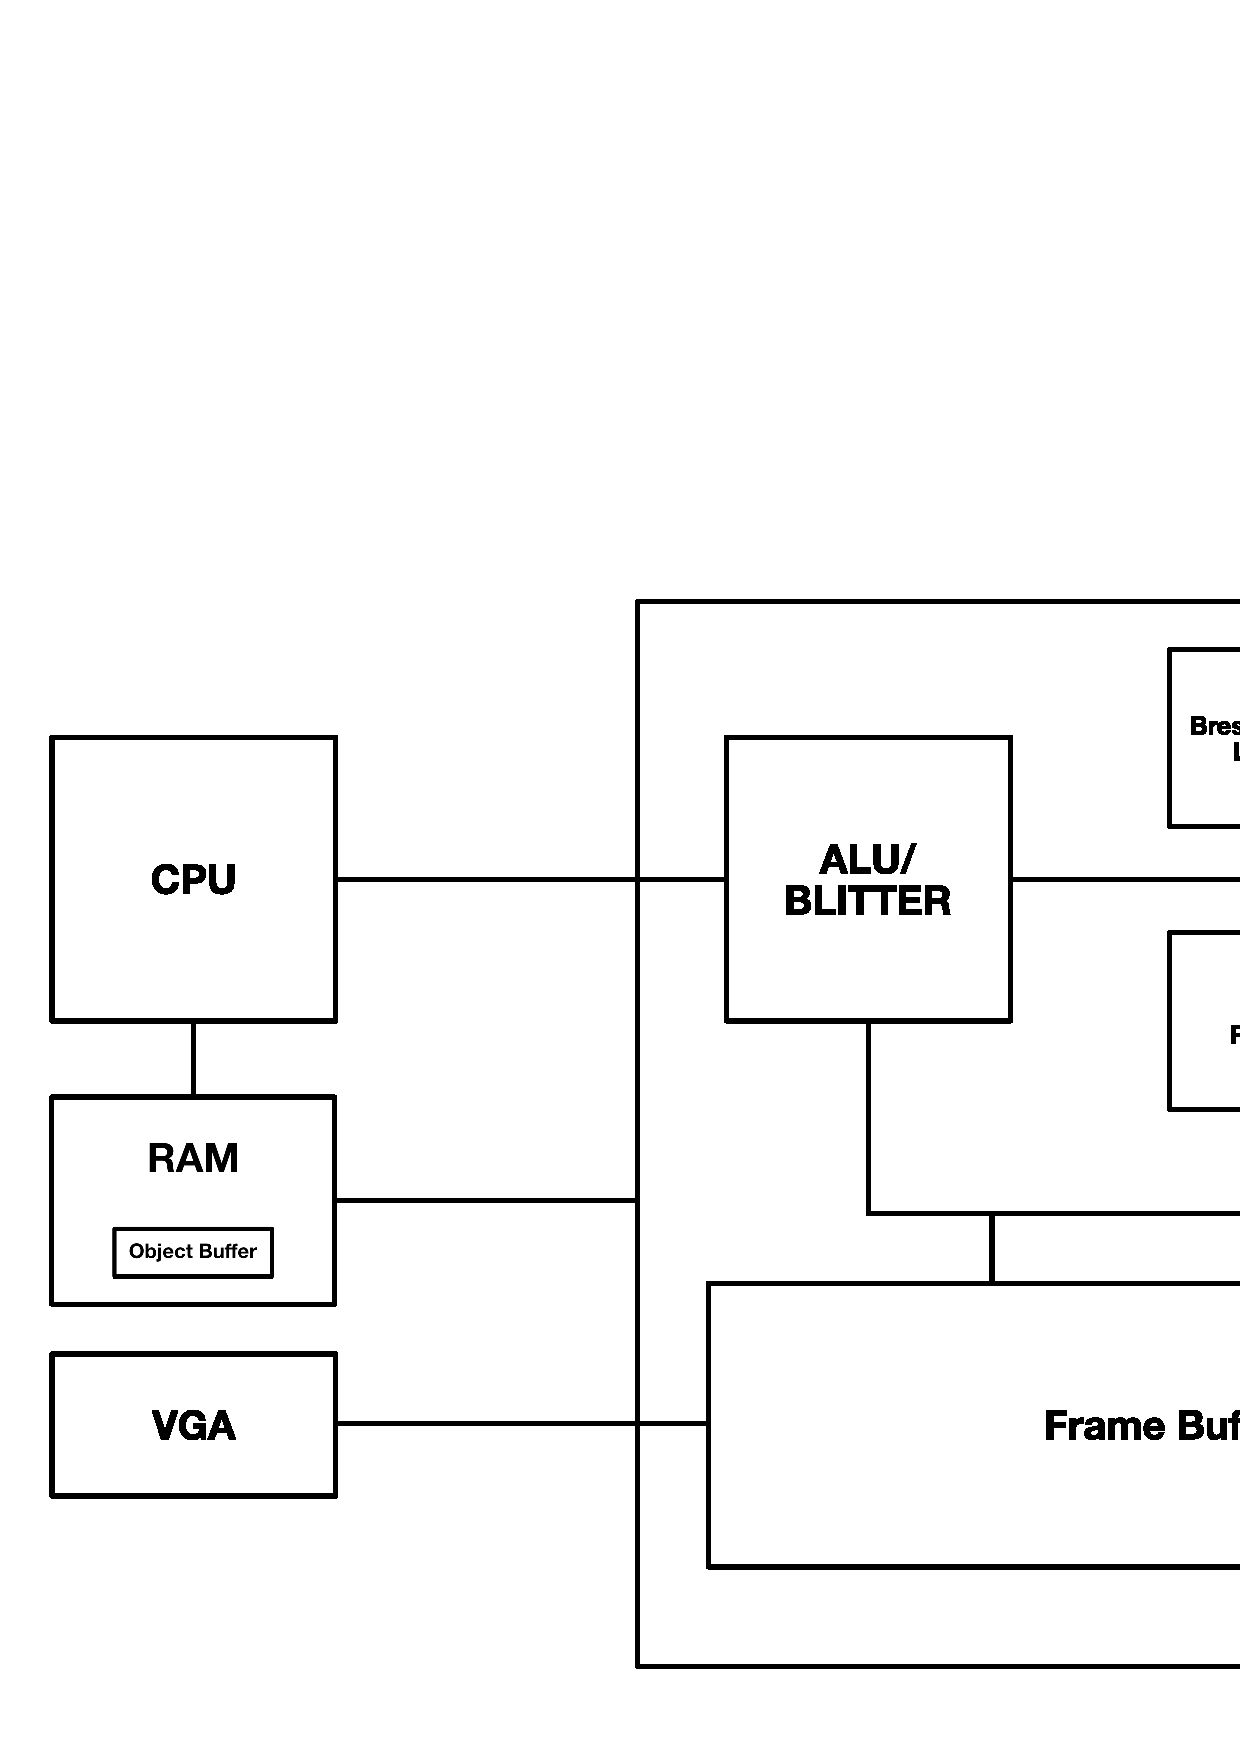
\includegraphics[width=0.5\textwidth]{coredesign}
	\caption{Graphical Design of the AEGIS Core }
	\label{img:coredes}
\end{figure}

For the communication between the CPU and the graphics accelerator, we use two AXI4 buses. The first one is a Axi4Shared for the communication with the CPU, and the second one is a Axi4readonly for the communication with the RAM.

When a write command is send over the AXI4 bus the graphics accelerator looks at the address. Is the address in the range of the double frame buffer, then it writes to it. Otherwise the address determines, what the graphics accelerator do. Further information he needs to operate get it from RAM at the address in the data value. 

\subsubsection*{Implementation}
\begin{itemize}
	\item is the main controll system, that is why is called mcp (tron)
	\item it has two state machine, the second one is a nested one
	\item it controlls both axi buses, the shared one as a slave and the readonly as a master
	\item the idle state waits until on the slave axi bus the following signal are set io.axicpu.sharedCmd.valid and he looks if the axi bus wants to read or write
	\item after that when the 25 bit is set it saves some data from the axi bus and goes to a wait state
	\item in the wait state it set the needed axi bus signals for the handshake and goes to the respones state
	\item here it set the neede signals for the responseand wait until the axi bus says its ok, after that it goes to the readdata state. or it goes to the switch state if a switch frame buffer is requested
	\item befor the switch case in the readdata is running, the nested state machine is activated
	\item the nested state machine is for the communication to the ram.
	\item it set the needed signals for the axi master bus, like how big is a word and the burst mode
	\item the read state is diveded in two stages the first one get the signals and the second one saves it into the temp variables
	\item the second state is divided into four states because we need different variables, and the sprite state saves the sprite directly to the framebuffer
	\item when all the data are read it goes to the exit state, we can have only one exitState int the hole state machine
	\item after the nested state machine is ready the readdata state determine which function we want
	\item after the function are ready it goes to the idle state.
	\item when the 23 bit is not set, the state machine read or write directly to the framebuffer. The programmer must keep track which framebuffer he want to read or write
\end{itemize}